\documentclass{beamer}

\usepackage{tikz}
\usepackage{tikzducks,tikzlings}

\setbeamertemplate{background canvas}{
  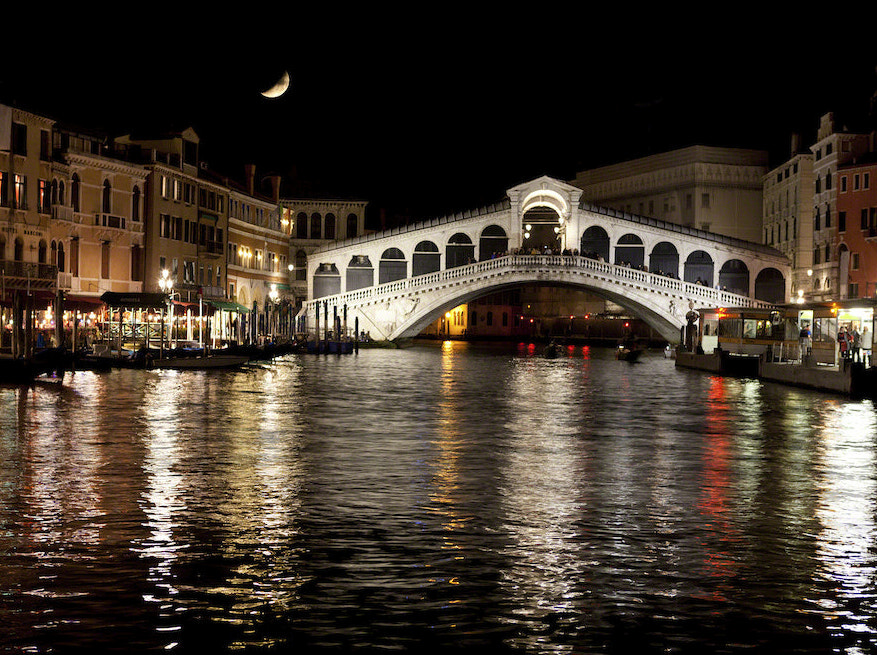
\includegraphics[height=\paperheight]{Rialto_Bridge_Grand_Canal_Venice_Italy_(104466307)}
}
\setbeamertemplate{navigation symbols}{}

\begin{document}

\begin{frame}
  \begin{tikzpicture}[remember picture, overlay]
    \begin{scope}[
      xshift=300-700*\thepage/20
    ]
      \begin{scope}[yshift=-2.7cm, xshift=7.5cm]
        \duck[
          body= yellow!70!brown!80!gray,
          stripes={\stripes[color=blue!70!darkgray!80!gray,rotate=-87,width=0.07,distance=0.12]},
          hat=white!80!gray,
          tshirt=white!80!gray,
          neckerchief=red!70!gray!80!gray,
          woggle=red!70!gray!80!gray
        ]
        %
        % adding red stripe to hat
        \fill[red!70!gray!80!gray,rotate=-15] (0.44,2.15) ellipse[x radius=0.37, y radius=0.08];
        \fill[red!70!gray!80!gray,rotate=-15] (0.07,2.15) rectangle (0.81,2.25);
        \fill[white!80!gray,rotate=-15] (0.44,2.25) ellipse[x radius=0.37, y radius=0.08];
        %
        \node at (-1.5,0) {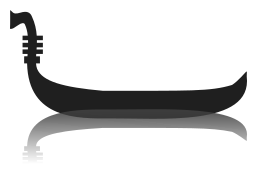
\includegraphics[width=9cm]{gondola}};
        %
        % boat oars
        \draw[black!70!gray,line width=4pt,line cap=round] (2,-1.5) -- (-0.5,2.3);
      \end{scope}
    \end{scope}
    \node at ([yshift=0.2cm]current page.south) {\color{white}\tiny Background image: \url{https://commons.wikimedia.org/wiki/File:Rialto_Bridge_Grand_Canal_Venice_Italy_(104466307).jpeg}};
  \end{tikzpicture}
	\pause[20]
\end{frame}	

\end{document}